\documentclass{report}
% PACKAGES
\usepackage[utf8]{inputenc}
\usepackage{mathtools} % math and figures
\usepackage{float} % make figure appear where we want with [H]
\usepackage{filecontents}
\usepackage[numbered,framed]{matlab-prettifier}
% these packages include more math symbols you might use
\usepackage{amsmath,amsfonts,amsthm,amssymb}


% PROJECT Specific Information to Fill Out
\newcommand{\LectureDate}{\today}
\newcommand{\LectureClassName}{Problem Set 3}
\newcommand{\LatexerName}{SeungWha Lee, Xinyuan Meng, Boyang Pan}
\author{\LatexerName}


% CONFIGURATIONS to make the report look better
\usepackage{setspace}
\usepackage{Tabbing}
\usepackage{fancyhdr}
\usepackage{lastpage}
\usepackage{extramarks}
\usepackage{afterpage}
\usepackage{abstract}

% In case you need to adjust margins:
\topmargin=-0.45in
\evensidemargin=0in
\oddsidemargin=0in
\textwidth=6.5in
\textheight=9.0in
\headsep=0.25in

% Setup the header and footer
\pagestyle{fancy}
\lhead{\LatexerName}
\rhead{\LectureDate}
\lfoot{\lastxmark}
\cfoot{}
\rfoot{Page\ \thepage\ of\ \pageref{LastPage}}
\renewcommand\headrulewidth{0.4pt}
\renewcommand\footrulewidth{0.4pt}
\renewcommand\thesection{\arabic{section}}
\renewcommand{\thesubsection}{\thesection.\Alph{subsection}}
\usepackage{color}

\title{\LectureTitle: Assignment 1}

\begin{document}
\maketitle
\newpage

\section{Exercise 1}
\subsection{Part A}
\begin{itemize}
	\item The means and deviations of each portfolio is given in the table below.
	\item The graphs display the relationship between standard deviations and the number of stocks. Theoretically, the standard deviation will decrease to a certain level as the number of stocks increases. The remaining standard deviation is the systematic risk in theory. My result is consistent with the theoretical expectation. In the graph, the standard deviation firstly goes down as the number of stocks increases, but it remains relatively constant after the number of stocks exceeds 20.
	\item In the graph, adding more and more stocks will not diversify away all of the standard deviation, because only idiosyncratic risk can be diversified away but systematic risk cannot.
\end{itemize}
\begin{table}[H]
	\centering
	\caption{The means and standard deviations of 4 equal-weight portfolios}
	\begin{tabular}{ccccc}\hline\hline
	Number of Stocks & 5 & 10 & 25 & 50 \\\hline
	Mean & 1.5164 & 1.2326 & 1.2119 & 1.2107 \\
	Standard Deviation & 9.8671 & 6.8118 & 5.5771 & 5.4281 \\ \hline
	\end{tabular}
\end{table}

\begin{figure}[H]
	\centering
	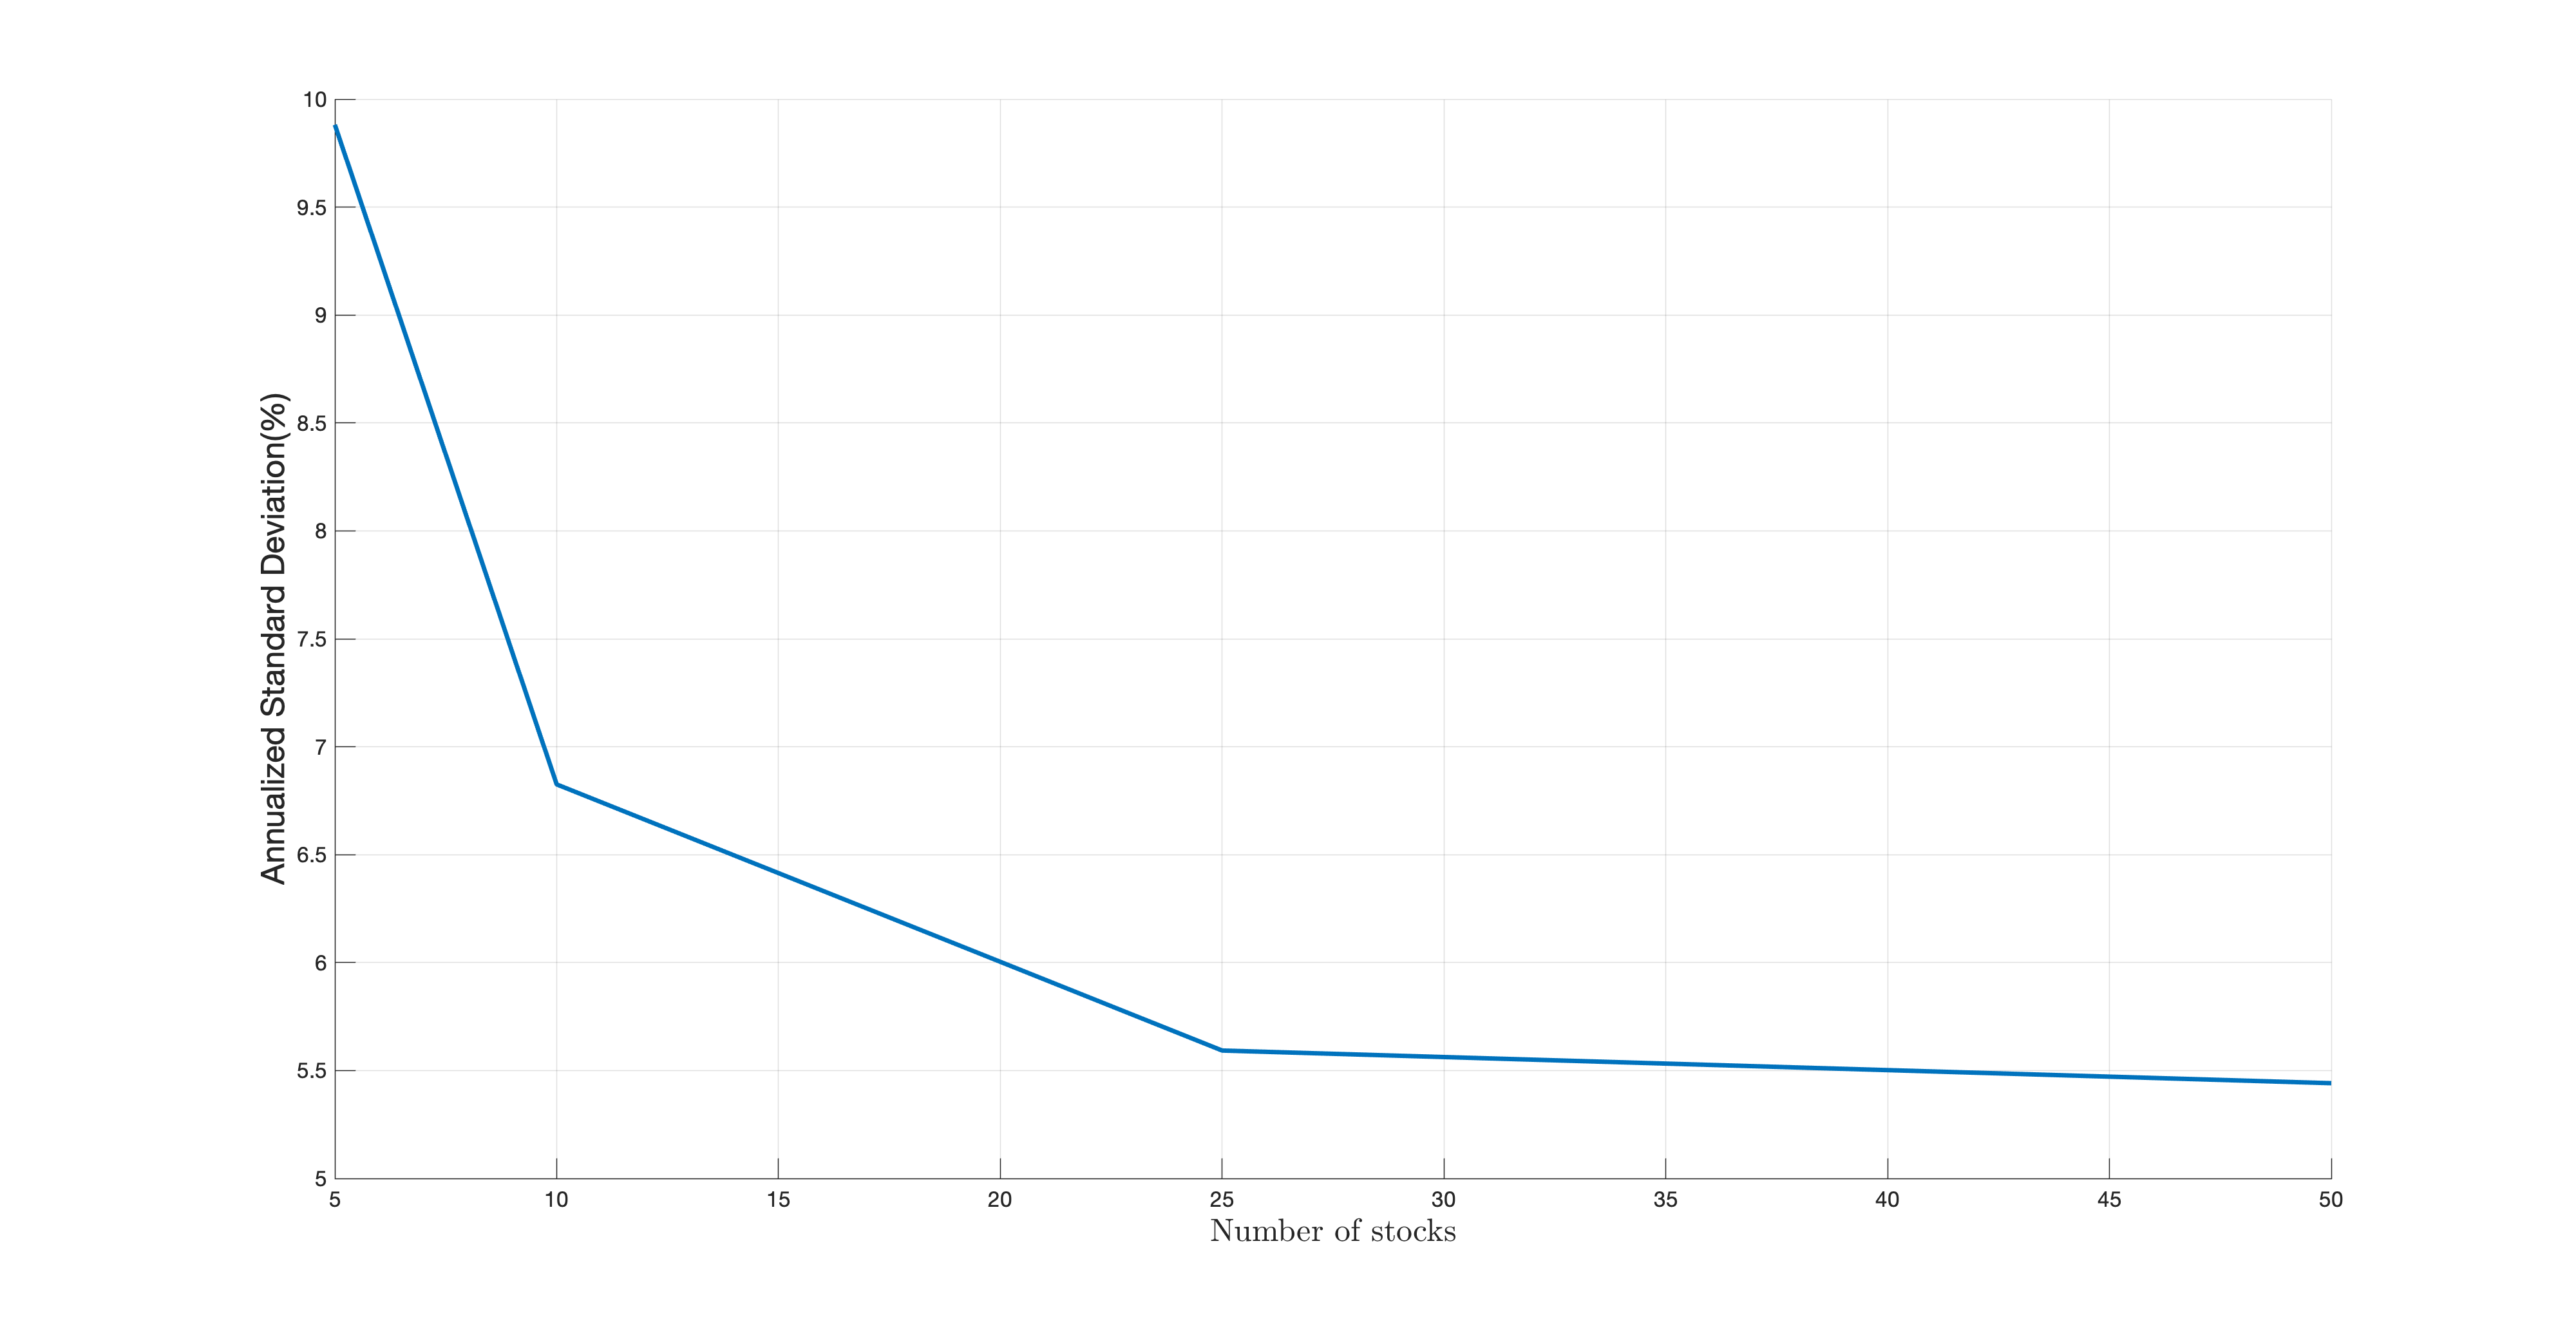
\includegraphics[width=1.0\textwidth]{figures/1A_sample}
	\caption{Estimated standard deviations for 4 equal-weight portfolios}
\end{figure}

\begin{figure}[H]
	\centering
	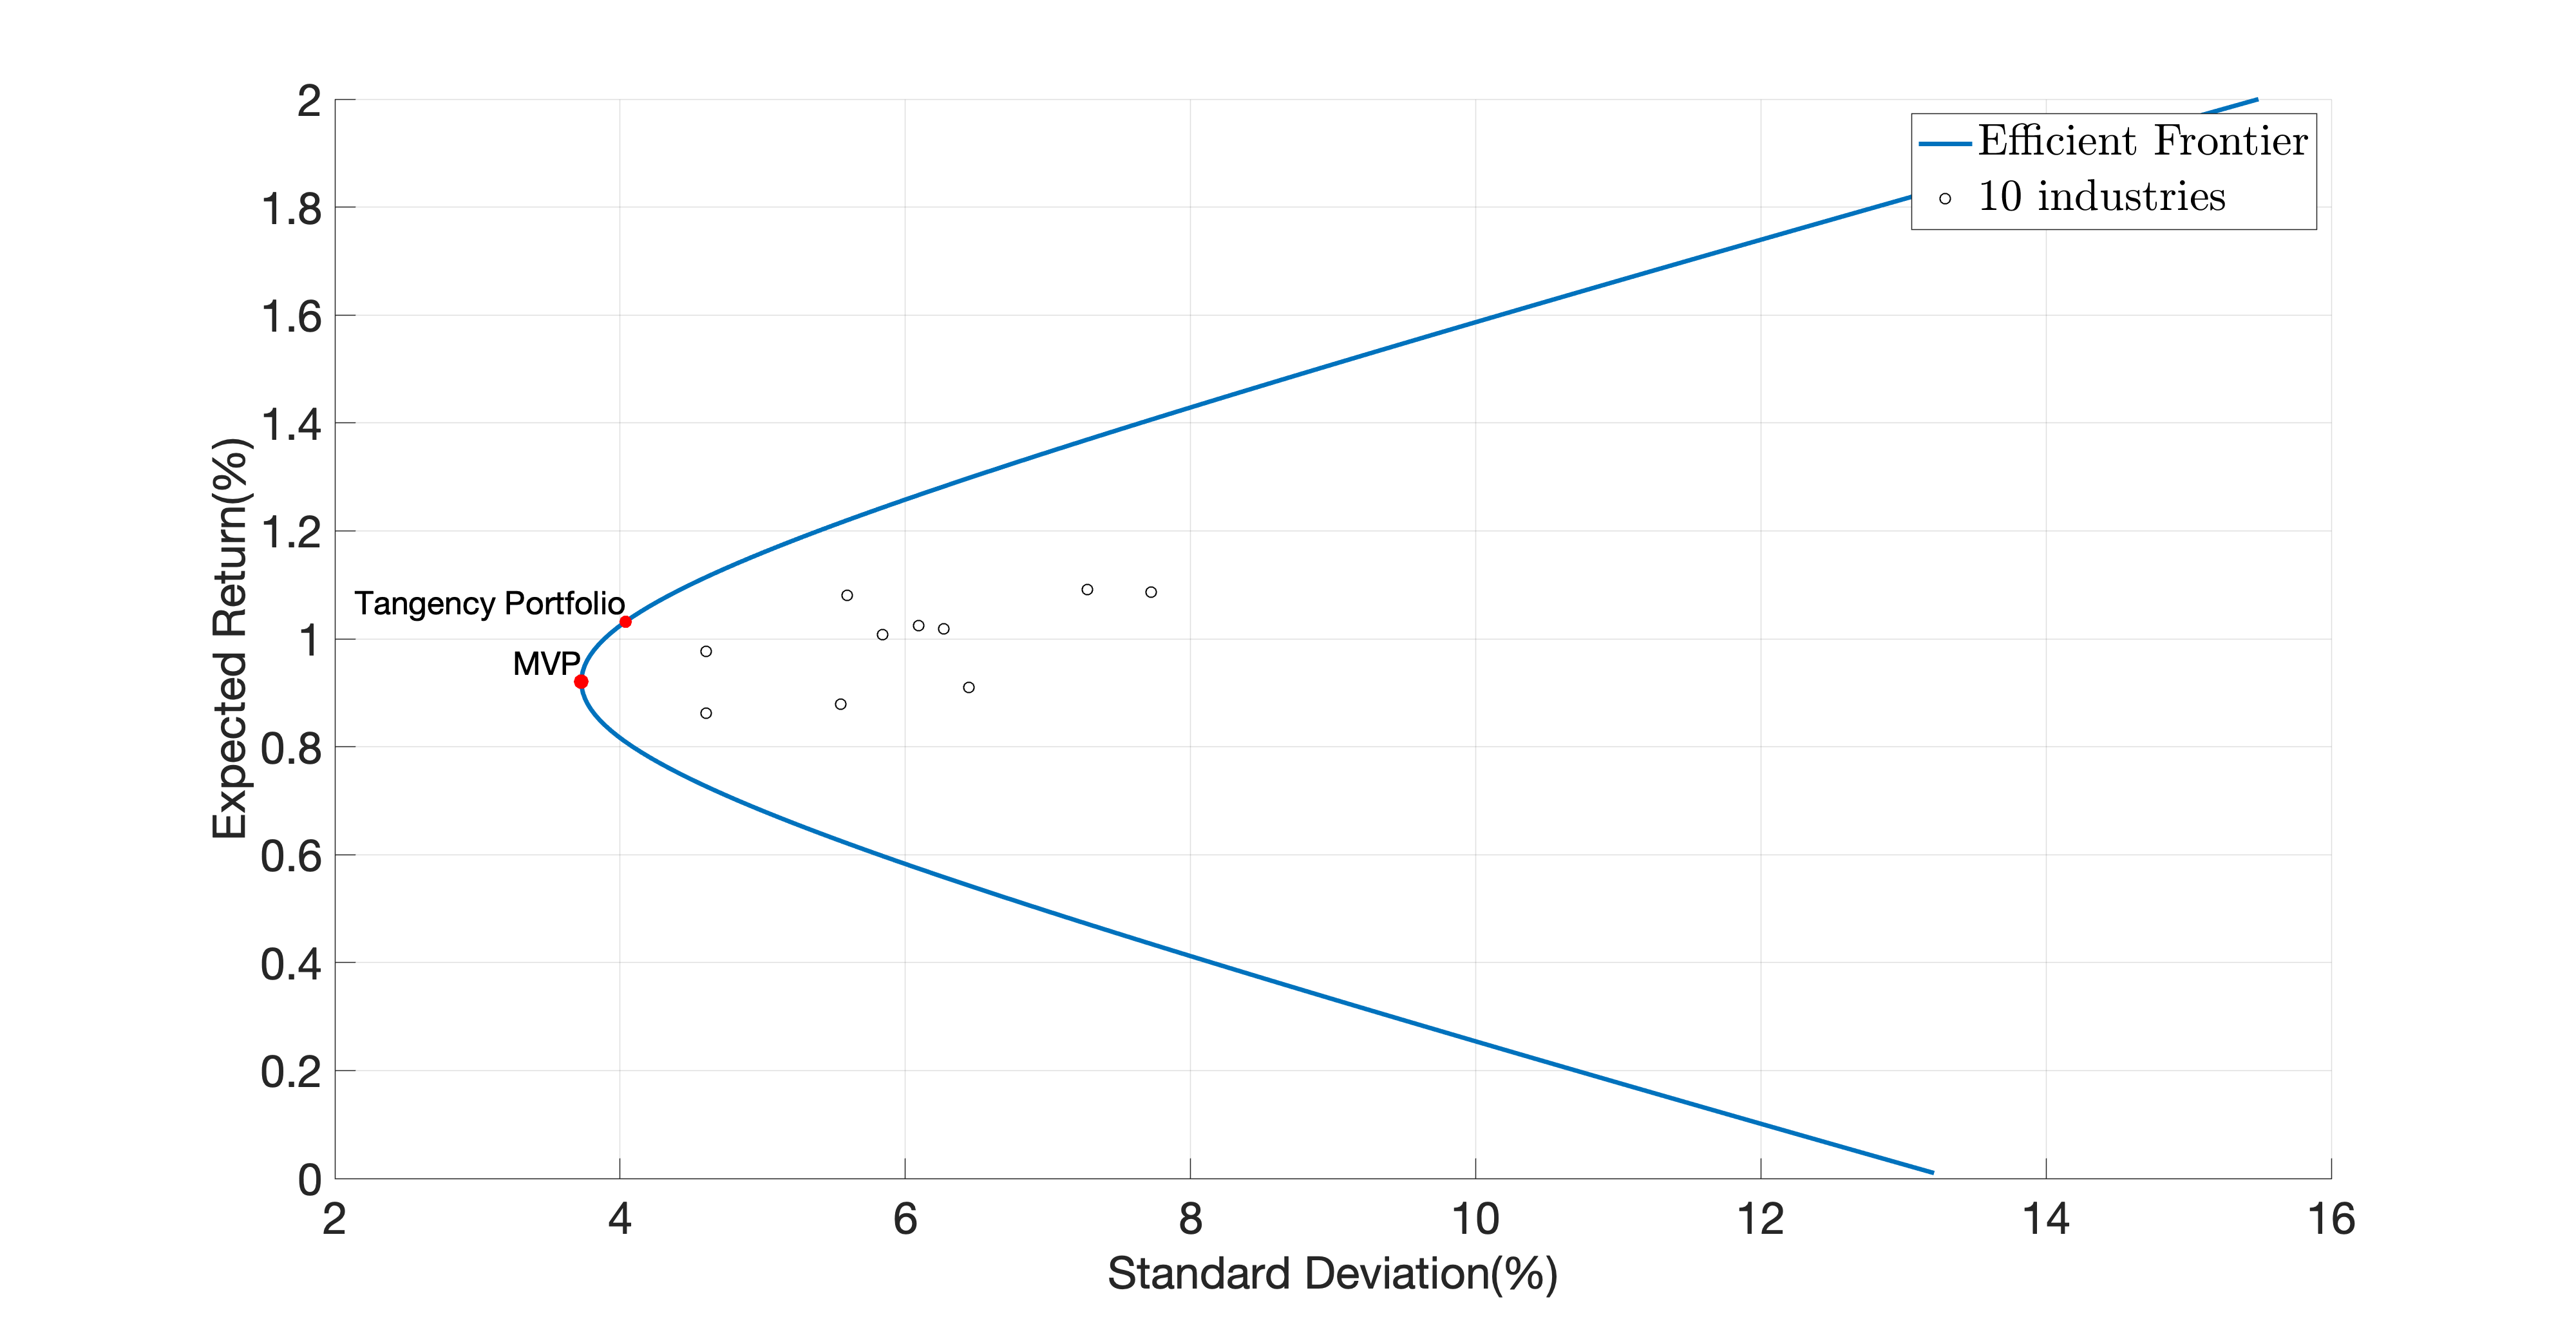
\includegraphics[width=1.0\textwidth]{figures/1A}
	\caption{Estimated standard deviations as a function of the number of stocks in the portfolio}
\end{figure}

\subsection{Part B}
To obtain the contribution of variance, I use the formula $\frac{\sum^{N}_{i=1}\sigma^2_{i}}{\sigma_{portfolio}^2}$. As for the contribution of covariance, it is (1 - contribution of variance).
\\The table and graph below shows the contribution of variance and covariance. In theory, covariance will play a more important role in a portfolio's volatility as the number of stocks increases. It is because adding more stocks into a portfolio will diversify away idiosyncratic risk of the stocks. 
\begin{table}[H]
	\centering
	\caption{The contribution of individual stocks' variance and covariance in 4 equal-weight portfolios}
	\begin{tabular}{ccccc}\hline\hline
	Number of Stocks & 5 & 10 & 25 & 50 \\\hline
	Variance & 46.57\% & 33.61\% & 16.31\% & 7.84\% \\
	Covariance & 53.43\% & 66.39\% & 83.69\% & 92.16\% \\ \hline
	\end{tabular}
\end{table}

\begin{figure}[H]
	\centering
	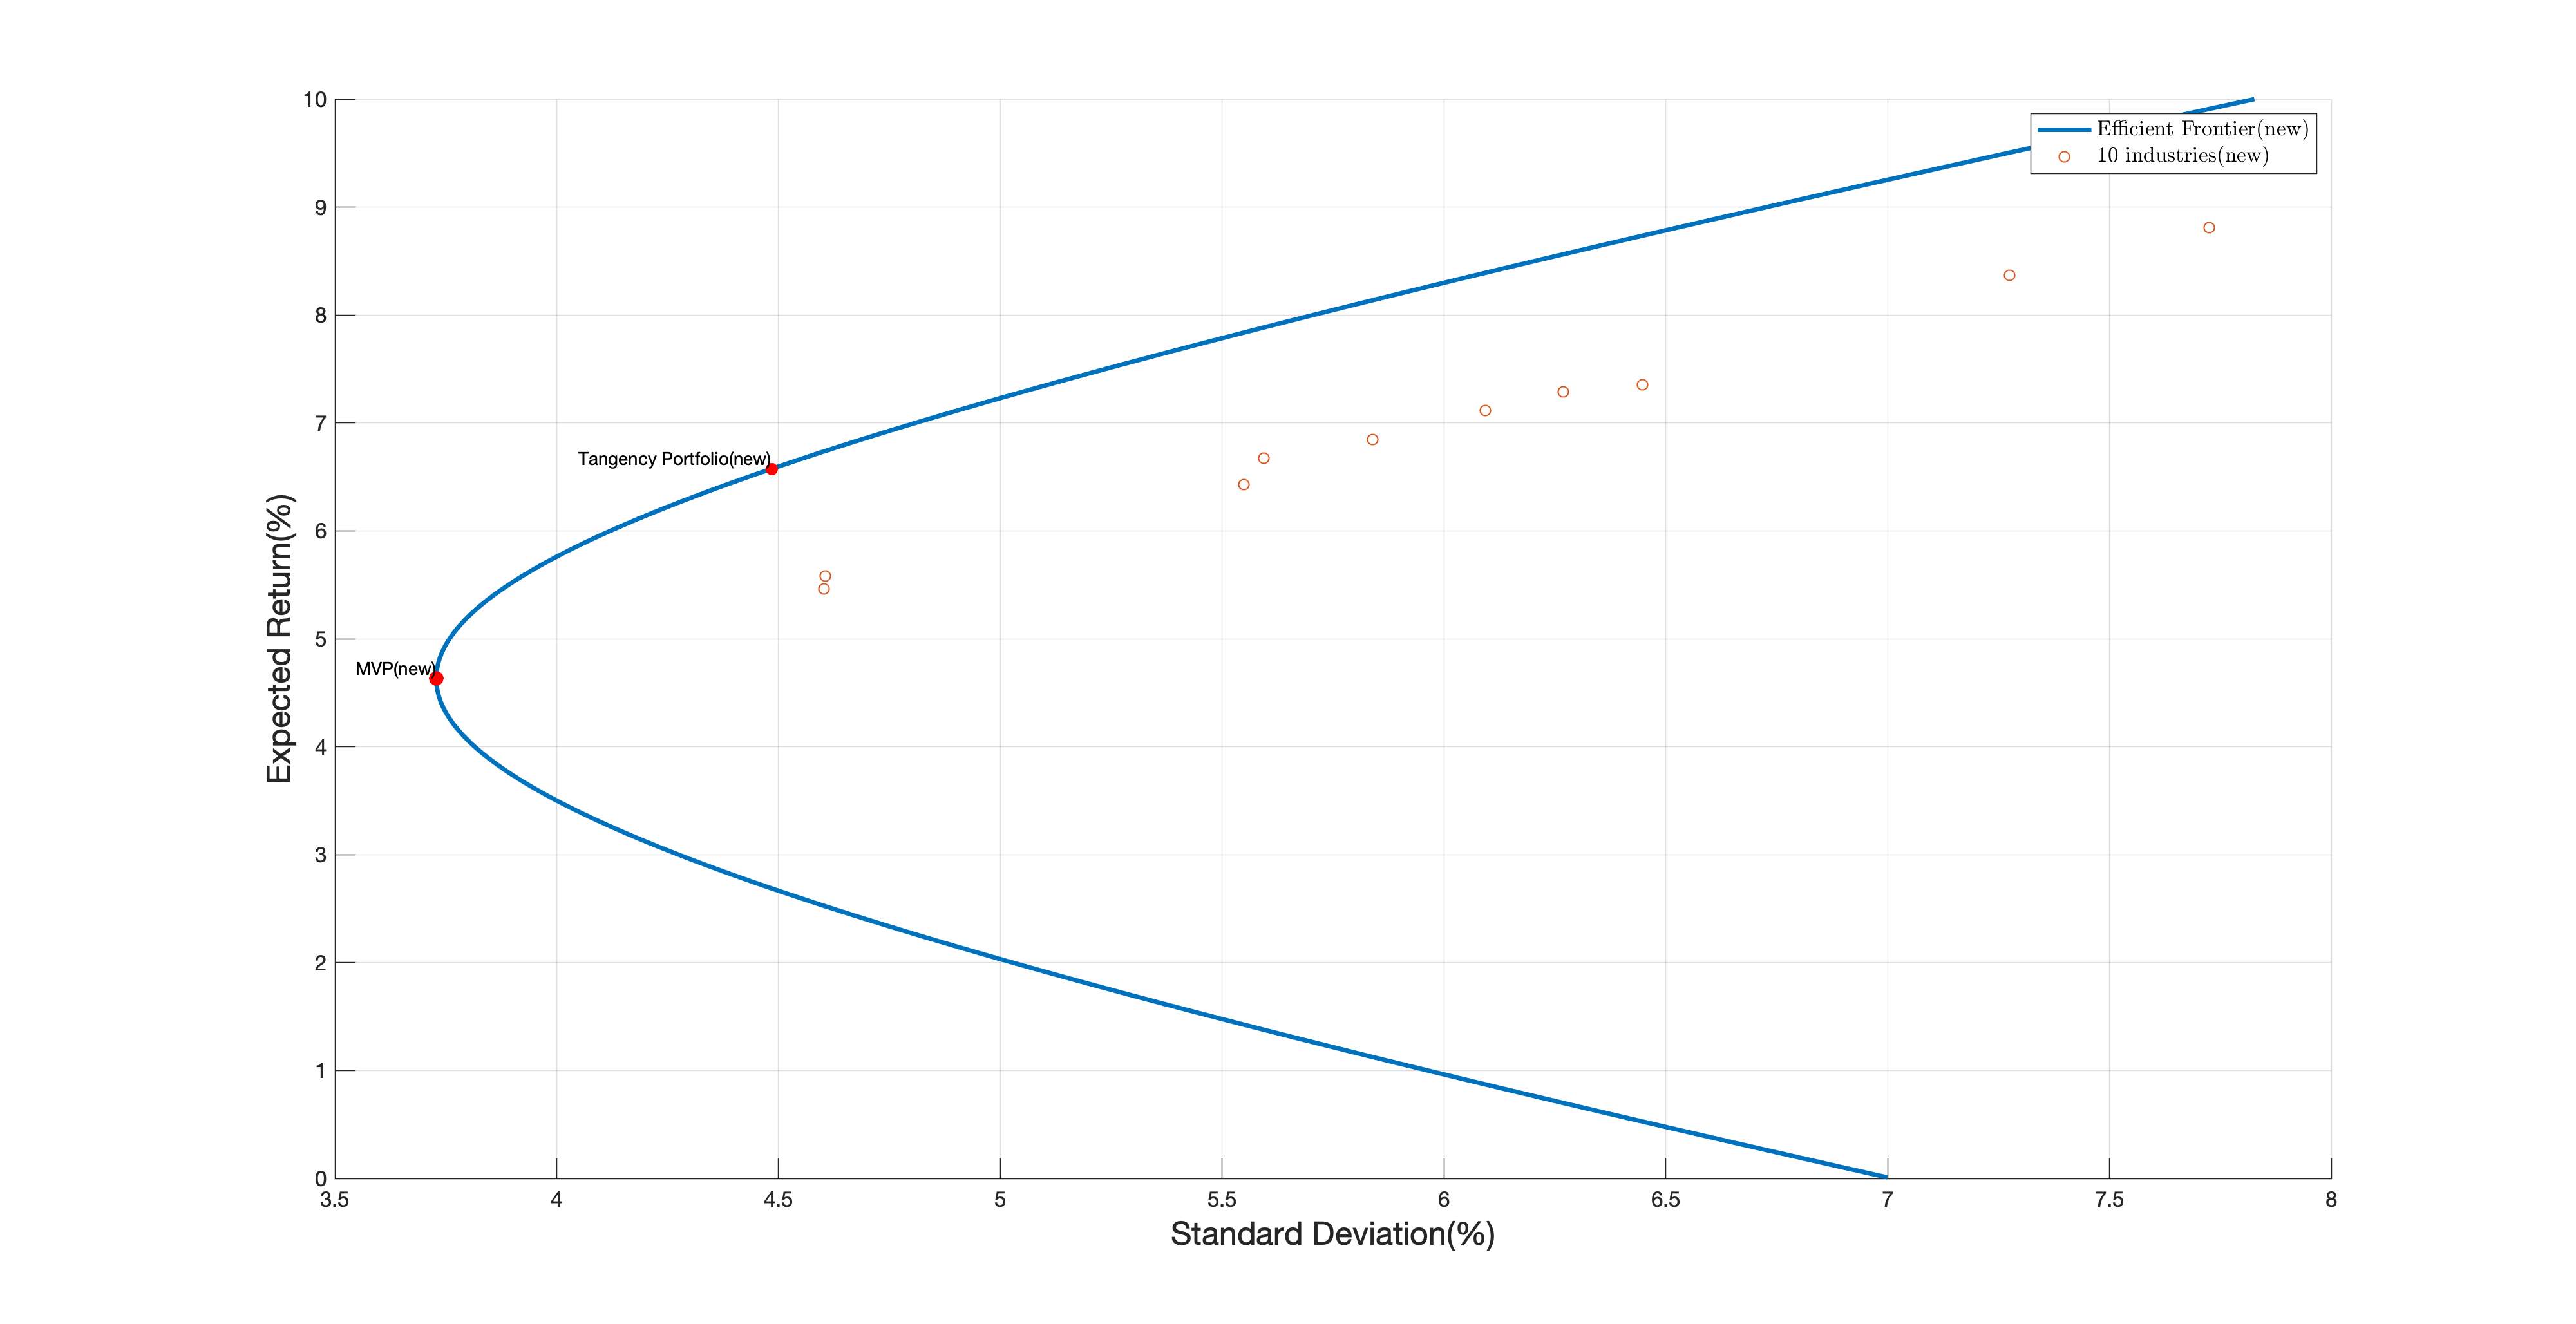
\includegraphics[width= 1.0\textwidth]{figures/1B}
	\caption{Contribution of variance and covariance as a function of the number of stocks in the portfolio}
\end{figure}

\subsection{Part C}
\begin{itemize}
	\item The variance of value-weighted portfolios is expected to be less relative to the equal-weighted portfolios. Because value-weighted portfolios give more weights to the stocks with high capital. These stocks have relatively lower variance, which results in a lower variance. 
	\item It might depend on the size of the portfolio. \\A portfolio's variance = $\sum_{i=1}^{N}Var(r_i) + \sum_{i=1}^{N}\sum_{j=1}^{N}cov(r_i,r_j)1_{\{ i\ne j\}}$. If a portfolio has only a few stocks, the idiosyncratic risk of each stock dominates the portfolio's variance. Therefore, a value-weighted portfolio will have a relatively low variance because those stable high-capital stocks are given more weights. If a portfolio has a great number of stocks, the portfolio's variance will be dominated by the covariances. Then, it depends on the covariances' signs and magnitudes, and how they cumulate or cancel off each other.
\end{itemize}

\subsection{Part D}
The test statistics should be $t_{stat} = \frac{\mu - \mu_0}{\sigma_{return}/\sqrt{n}}$, where $\mu_0$ is 0 given the null hypothesis and n is 180, which is the sample size.
\begin{itemize}
	\item For each portfolio, we have 180 observations, so the test statistics are t-statistics and follow t distribution. 
	\item The test statistics are given in the table below. Because the z-stat's of these portfolio are larger than 1.96, we reject the null hypothesis that each of the mean returns on the portfolios is different from zero at a 5\%  level.
\end{itemize}
\begin{table}[H]
	\centering
	\caption{The test statistics of 4 equal-weight portfolios}
	\begin{tabular}{ccccc}\hline\hline
	Number of Stocks & 5 & 10 & 25 & 50 \\\hline
	test-statistics & 2.0619 & 2.4278 & 2.9153 & 2.9924 \\ \hline
	\end{tabular}
\end{table}

\subsection{Part E}
I use the Jarque-Bera test to test if a portfolio's returns follow a normal distribution. \\
JB test statistics = $n(\frac{v^2}{6}+\frac{(k-3)^2}{24})$, where n = observations, v = skewness, k = kurtosis.\\
We reject the null hypothesis at 5\% significance level with a critical value of 5.6490. \\
\begin{itemize}
\item The JB test statistics for each portfolio is given in the table below. All three test statistics exceed 5.6490, so all the portfolios do not follow a normal distribution.
\end{itemize}
\begin{table}[H]
	\centering
	\caption{JB test statistics}
	\begin{tabular}{cccccl}\hline\hline
 &Normal Distribution & \multicolumn{2}{c}{Equity Portfolio} & \multicolumn{2}{c}{market portfolio} \\\hline
Number of stocks & &1 & 50 & \multicolumn{2}{c}{} \\\hline
Studentized range &$\infty$& 6.2755 & 7.7113 & \multicolumn{2}{c}{6.6446}\\
Skewness &0& -0.1820 & -0.5244 & \multicolumn{2}{c}{-0.6657}\\
Kurtosis &3& 4.0297 & 5.3941 & \multicolumn{2}{c}{4.3339}\\
test statistics &5.6490& 8.9459 & 51.2367 & \multicolumn{2}{c}{26.6396}\\\hline
\end{tabular}
\end{table}

\subsection{Part F}
\begin{table}[H]
	\centering
	\caption{Regression the returns of the stocks on the market portfolio}
	\begin{tabular}{ccccl}\hline\hline
 	& Slope & Intercept & $R^2$ \\\hline
	TXN & 1.3995 & -0.0987 & 44.04\% \\
	ISRG & 1.3993 & 2.5118 & 12.97\% \\
	CIEN & 2.5154 & -1.4257 & 35.95\% \\
	BHI & 1.2665 & -0.0037 & 32.04\% \\
	WDC & 1.5840 & 2.1986 & 17.95\% \\
	CAH & 0.6487 & 0.3354 & 19.39\% \\
	CCI & 1.5545 & 0.7690 & 26.56\% \\
	BBT & 0.7211 & 0.1996 & 17.60\% \\
	TAP & 0.7239 & 0.5382 & 18.16\% \\
	VMC & 1.1185 & 0.3335 &31.30\% \\\hline
\end{tabular}
\end{table}	
\subsubsection{Part 1}
The slope coefficients of this model indicate the sensitivity of stocks return to the market. For example, when the return of the market index increases by 1\%, the return of TXN is expected to increase 1.3995\%.
\subsubsection{Part 2}
The intercepts are the expected returns of stocks that are not affected by the market return, or equivalently, it is the expected returns of stocks when the market return is 0. 
\subsubsection{Part 3}
$R^2$ indicates how much percent of a stock's return can be explained by the return of the market portfolio. From the table above, we can find some regression models have strong explanatory power, such as TXN and CIEN, while some have low explanatory power, such as ISRG and BBT. A low $R^2$ means the return of a stock can hardly be explained by the return of the market portfolio and more factors should be added to the model.

\newpage
\section{Part 2}
\subsection{Part a}
The annualized volatility estimates on TXN and the market index are displayed in the graphs below. The estimates by using the one-year samples is more volatile than the full samples. The two possible reasons are that:
\begin{itemize}
\item An estimate with a larger sample size has a more accurate estimate than the one with a smaller sample size. Because the method 1 has full samples while the method 2 has only 12 samples, the method 1 has a more stable and accurate estimation of the standard deviation compared to the method 2.
\item The volatility is time-varying over time, so the estimates by the method 2 move around all the time. The estimates by the method 1 is smoother because the variation of the standard deviation is mitigated over a long time horizon.
\end{itemize}
\begin{figure}[H]
	\centering
	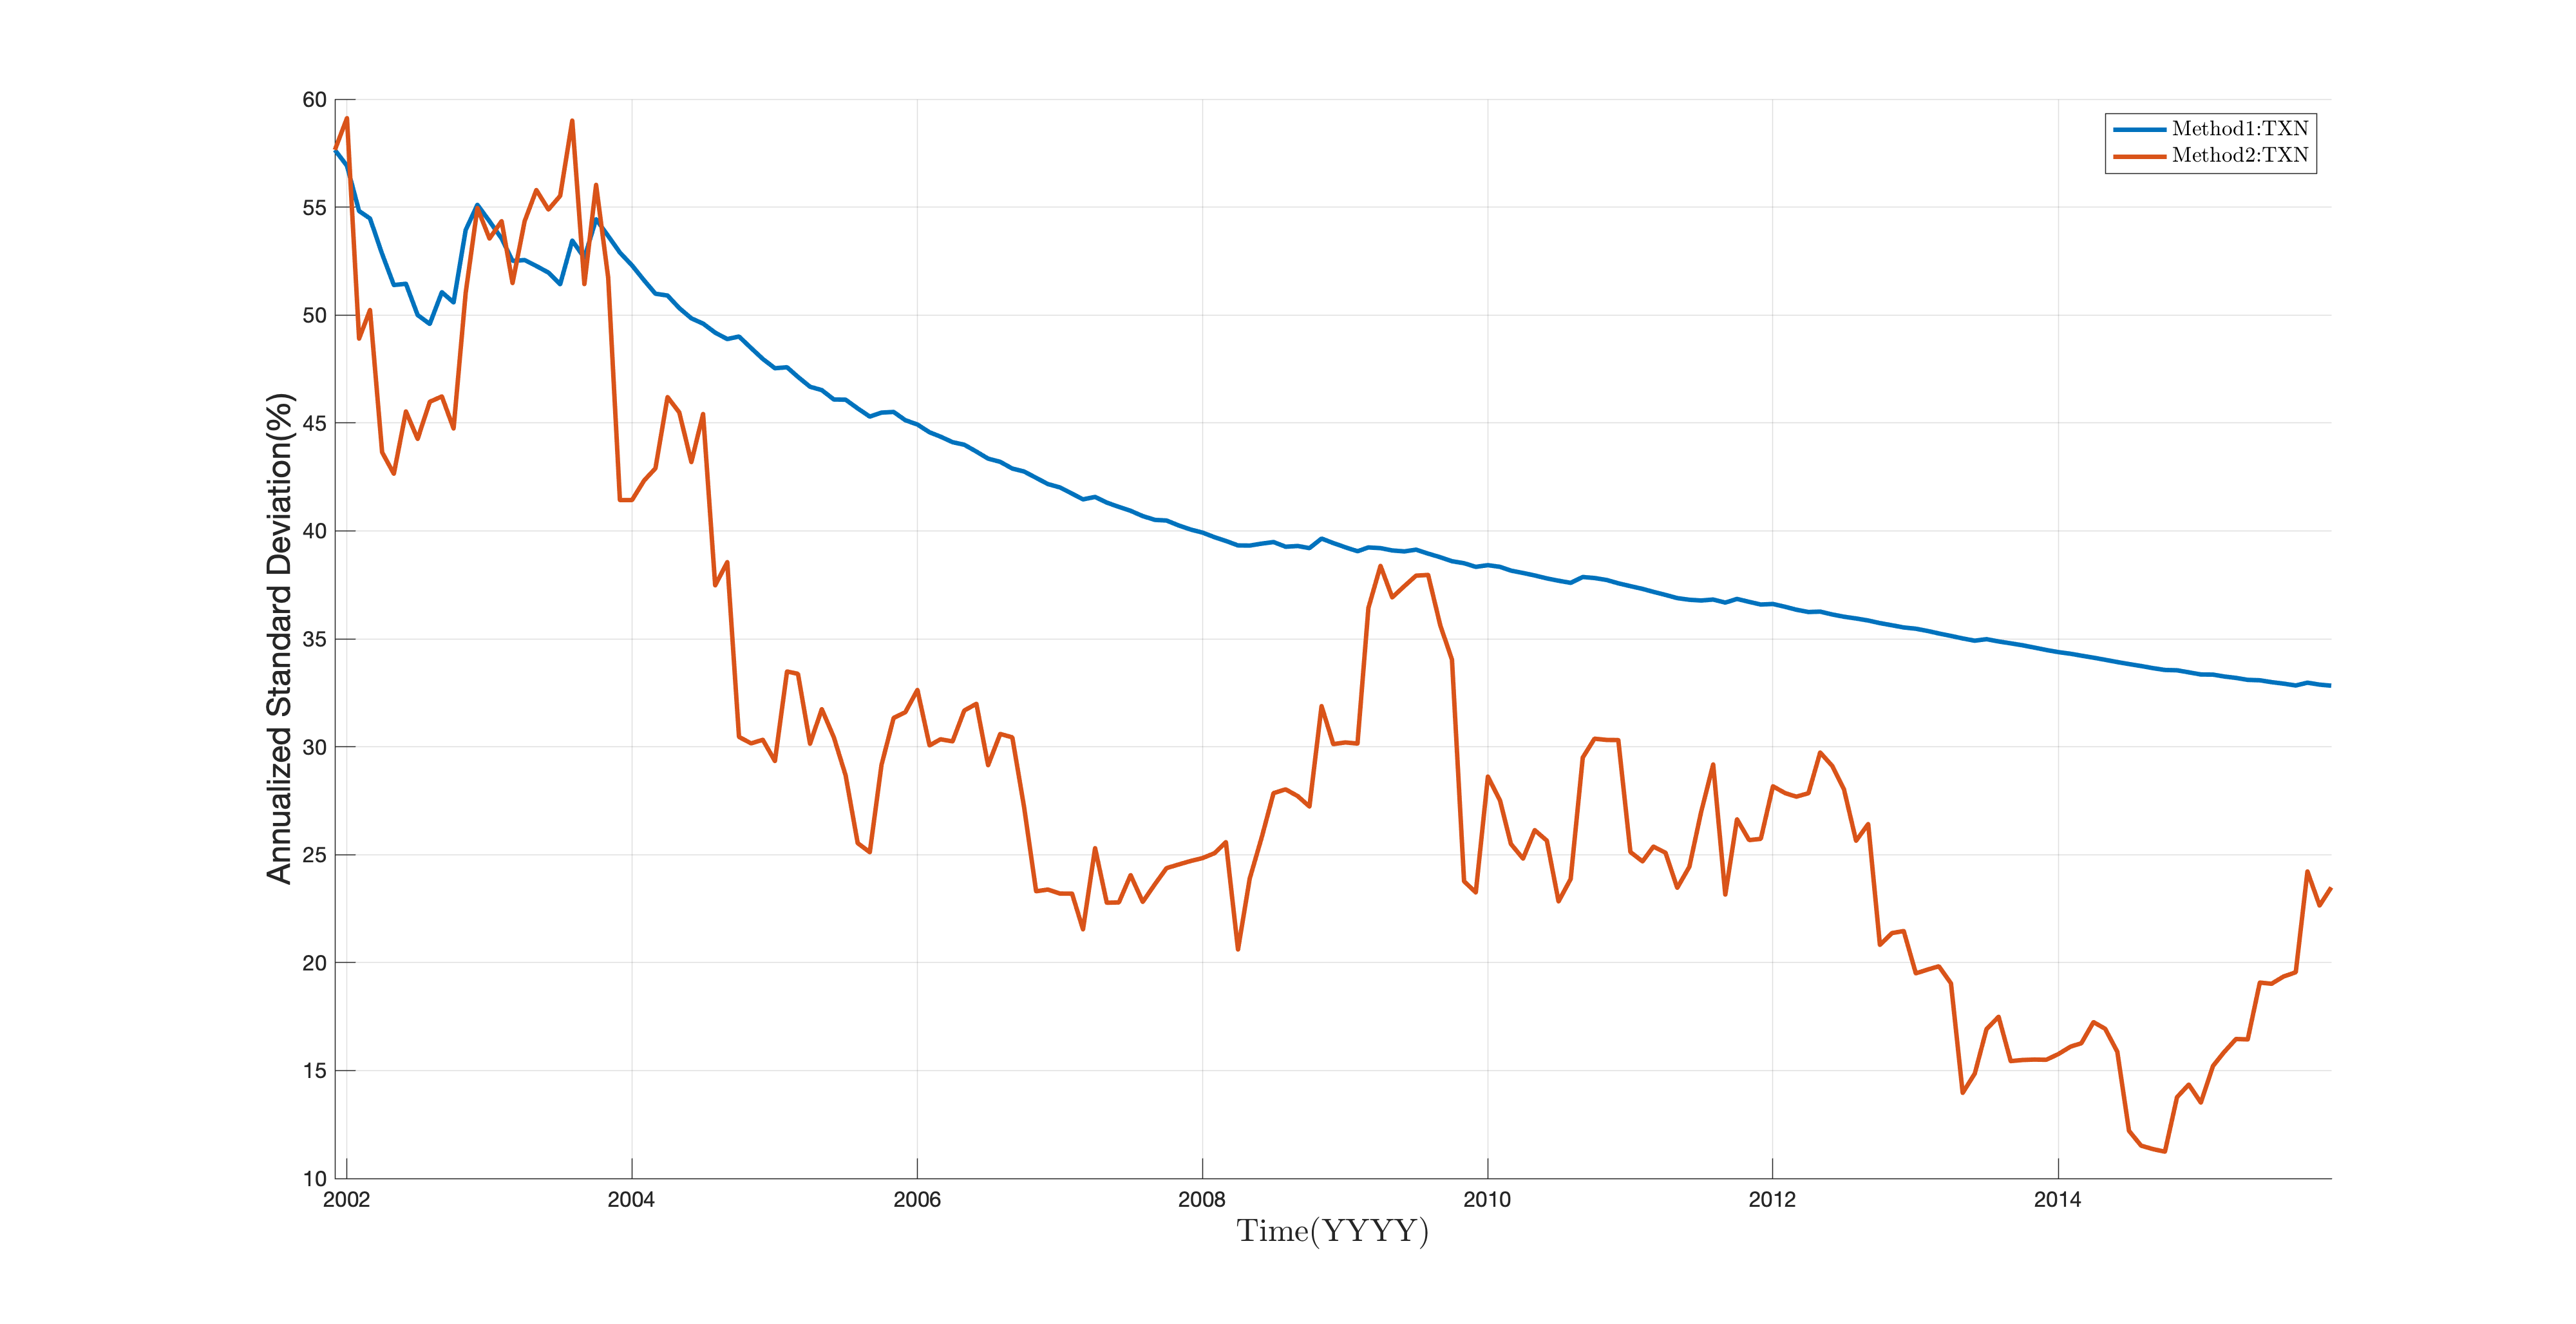
\includegraphics[width=0.8\textwidth]{figures/2A_TXN}
	\caption{Annualized standard deviations with 2 methods (TXN)}
\end{figure}

\begin{figure}[H]
	\centering
	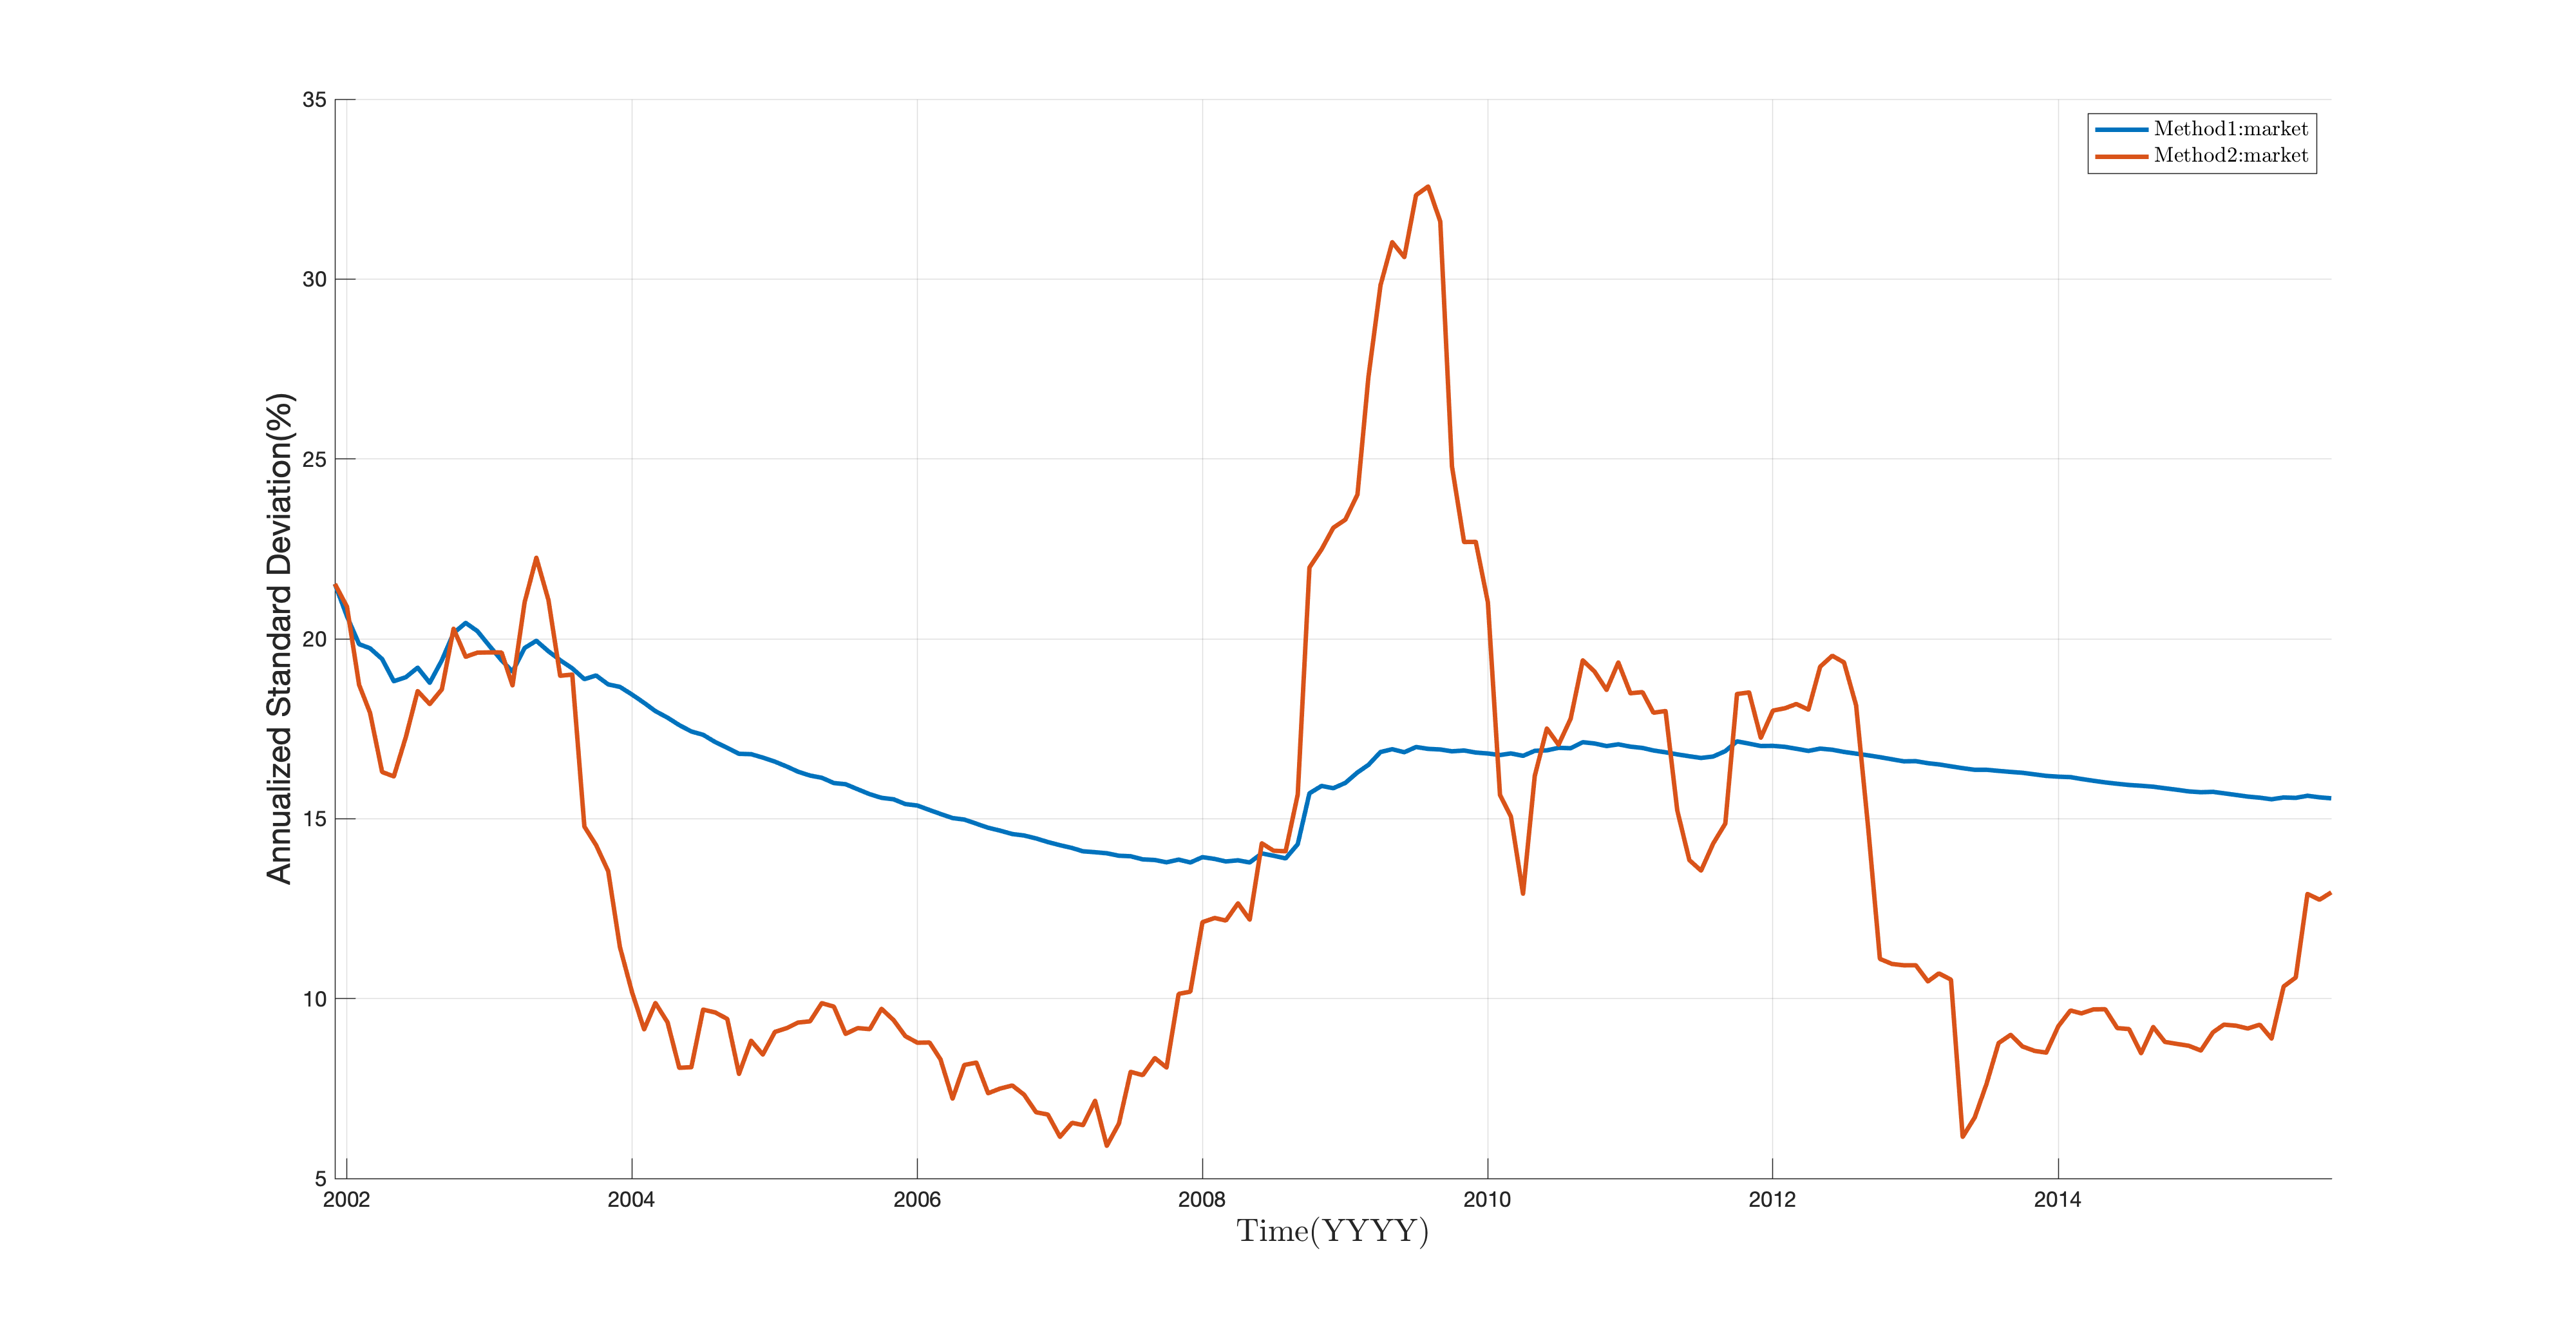
\includegraphics[width=0.8\textwidth]{figures/2A_mkt}
	\caption{Annualized standard deviations with 2 methods (Market Index)}
\end{figure}

\subsection{Part b}
The OLS beta estimates using the given methods are displayed below. The one-year estimates shows a more volatile pattern relative to the full-sample estimates. The possible explanations to this phenomenon are that :
\begin{itemize}
\item the different sample sizes for estimation result in a less accurate estimates of the one-year method and a more accurate estimates of the full-sample method. Because full-sample method use a larger sample size, it produces a more accurate and stable estimates.
\item the betas are time-varying over time, so the estimates by the method 2 is volatile, but the estimates by the method 1 is smoothened because the variation of the standard deviation is mitigated over a long time horizon.
\end{itemize}
\begin{figure}[H]
	\centering
	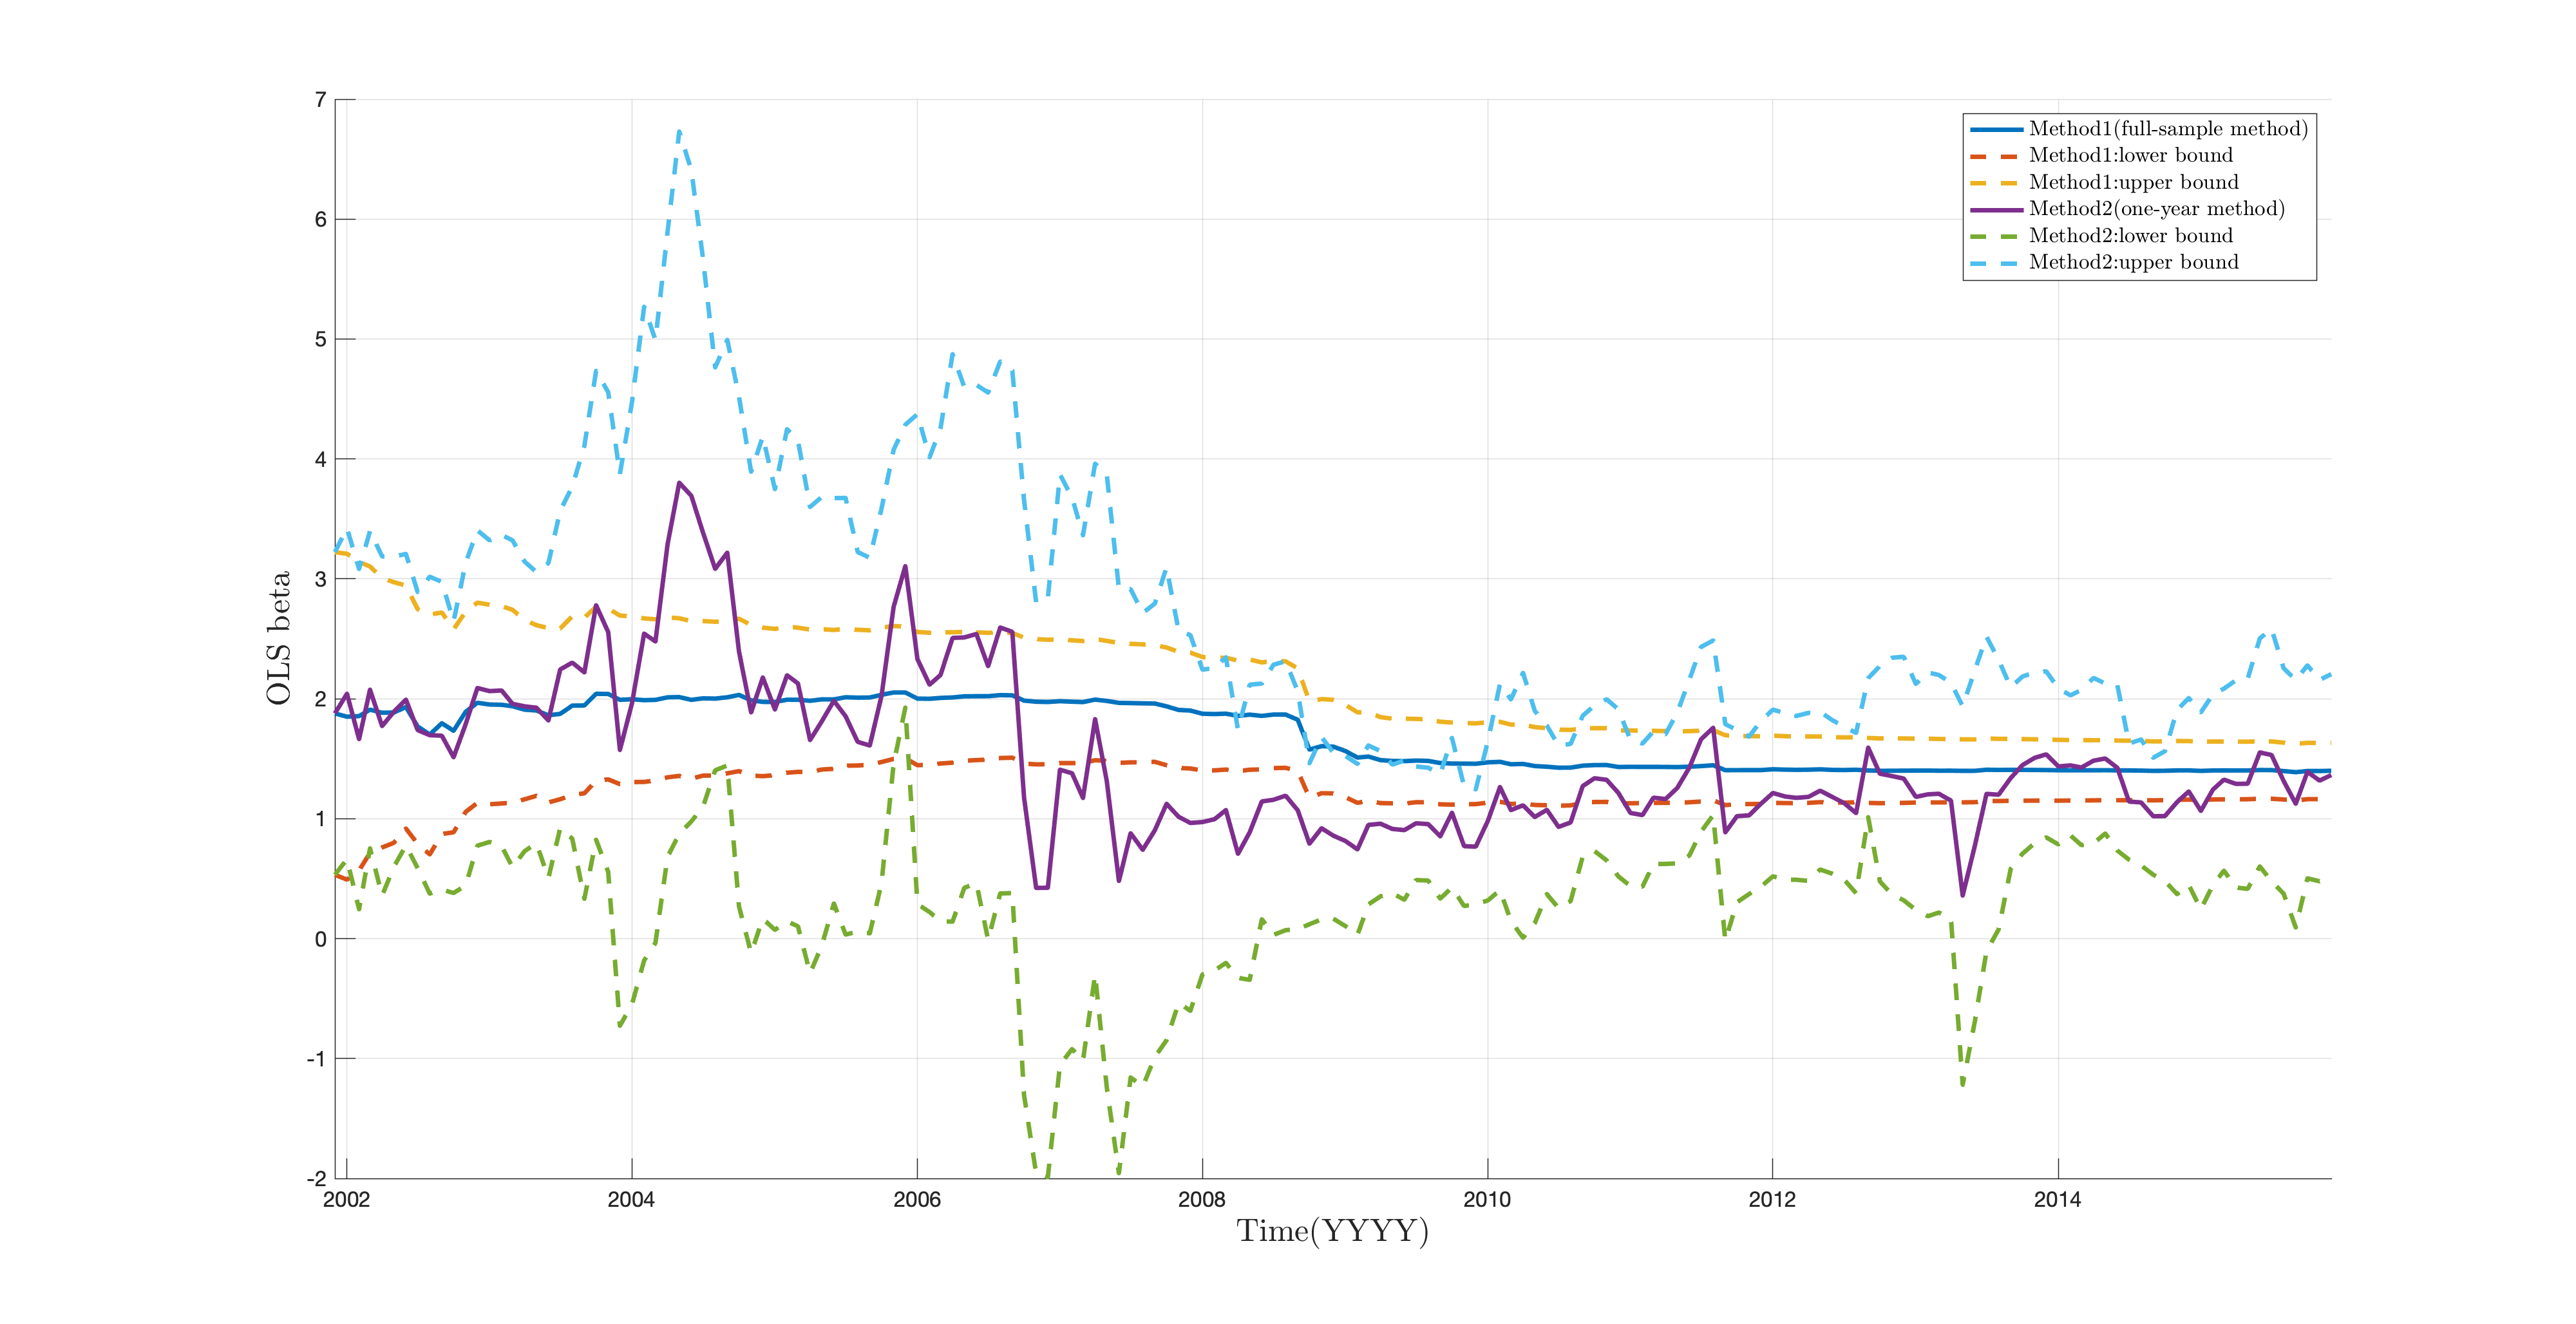
\includegraphics[width=0.9\textwidth]{figures/2B}
	\caption{OLS Betas and other confidence interval}
\end{figure}
\end{document}